\documentclass{jlreq}

\usepackage{amsmath, amssymb}
\usepackage{enumerate}
\usepackage{tikz}
\usepackage{listings, xcolor}
\usepackage{booktabs} % 綺麗な横線を引くため
\usepackage{float}    % 表の配置を固定するため
\usepackage{pdfpages}

\lstset{
  basicstyle = {\ttfamily}, % 基本的なフォントスタイル 
  frame = {tbrl}, % 枠線の枠線。t: top, b: bottom, r: right, l: left
  breaklines = true, % 長い行の改行
  numbers = left, % 行番号の表示。left, right, none
  showspaces = false, % スペースの表示
  showstringspaces = false, % 文字列中のスペースの表示
  showtabs = false, % タブの表示
  keywordstyle = \color{blue}, % キーワードのスタイル。intやwhileなど
  commentstyle = {\color[HTML]{1AB91A}}, % コメントのスタイル
  identifierstyle = \color{black}, % 識別子のスタイル 関数名や変数名
  stringstyle = \color{brown}, % 文字列のスタイル
  captionpos = t % キャプションの位置 t: 上、b: 下
}

\title{実験に対するデータ解析}
\author{情報学群2年 1280391\\ 細川 夏風}
\date{\today}

\begin{document}

  \maketitle


  \section{目的}
  近年,情報化社会により多くの情報が脳に届けられる.これによる認知負荷やあるサービスの理解の易さなどに多くの差が見られる.これらに対するサービスの質を向上させるための脳の認知の差異を明らかことを目的に実験を行う.

  \section{内容}
  \subsection*{使用技術}
  実験には以下の目的で以下のソフトウェアを用いた.
  \begin{enumerate}[(1). ]
    \item \verb|Pyschopy|: 実験環境の作成
    \item \verb|MATLAB|: 画像処理とデータ分析
    \item \verb|Excel|, \verb|Goole|スプレッドシート: データ分析とデータの格納
    \item \verb|Python|, \verb|R|: データ分析のためのプログラミング言語
    \item \verb|ImageJ|: 写真について様々な色覚の状態から確認できるソフトウェア
  \end{enumerate}
    それぞれのデータ分析の手法ごとにまとめる.
    \subsection*{第$1$回 ストループ効果}
    ストループ効果とは,単語の意味と色が一致しない場合,色を答えるのに時間がかかる現象をいう.この際,誤答の試行についてはデータ分析には含めない.誤答についても分析に加えてしまうと,提示された単語の意味や色に関係なく素早く入力し意図的にこの現象を否定することが可能になっているからである\cite{stroop}.

    \subsection*{第$2$回 統計的仮説検定}
    統計的仮説検定とは,仮説を立て母集団から取り出した標本から,その真偽を判定することをいう.考えられる全体を仮説の対象として考え,まず成り立たないと思われる仮説を帰無仮説として立て,その残りを対立仮説とする.そして,帰無仮説が棄却されたら採択される仮説が対立仮説である\cite{step}.

    \subsection*{第$3$回 主観評価実験}
    主観評価実験とはそれぞれのユーザの主観評価をいくつかの方法で測定する方法である.今回私たちが用いたのは,リッカート尺度という方法である.段階的な選択肢で,回答してもらう方法である.今回私たちは$5$段階で評価を行っている.

    \subsection*{第$4$回 ノンパラメトリック検定}
    ノンパラメトリック検定とは,母集団の分布の形が特定の仮定をおかないことをいう.逆に母集団の形が特定の形,正規分布であることを仮定することをパラメトリック検定という.ノンパラメトリック検定は外れ値の影響が少なく,比較的頑健であるとされている\cite{nonparametric}.

    \subsection*{第$5$回 カラーユニバーサルデザイン}
    カラーユニバーサルデザインとは,色覚の多様背に配慮し,すべての人に利用しやすい色のデザインを提供するデザイン方法のことをいう.
    
  \section{結果}
  \subsection*{第$1$回}
  \begin{figure}[hbp]
    \centering
    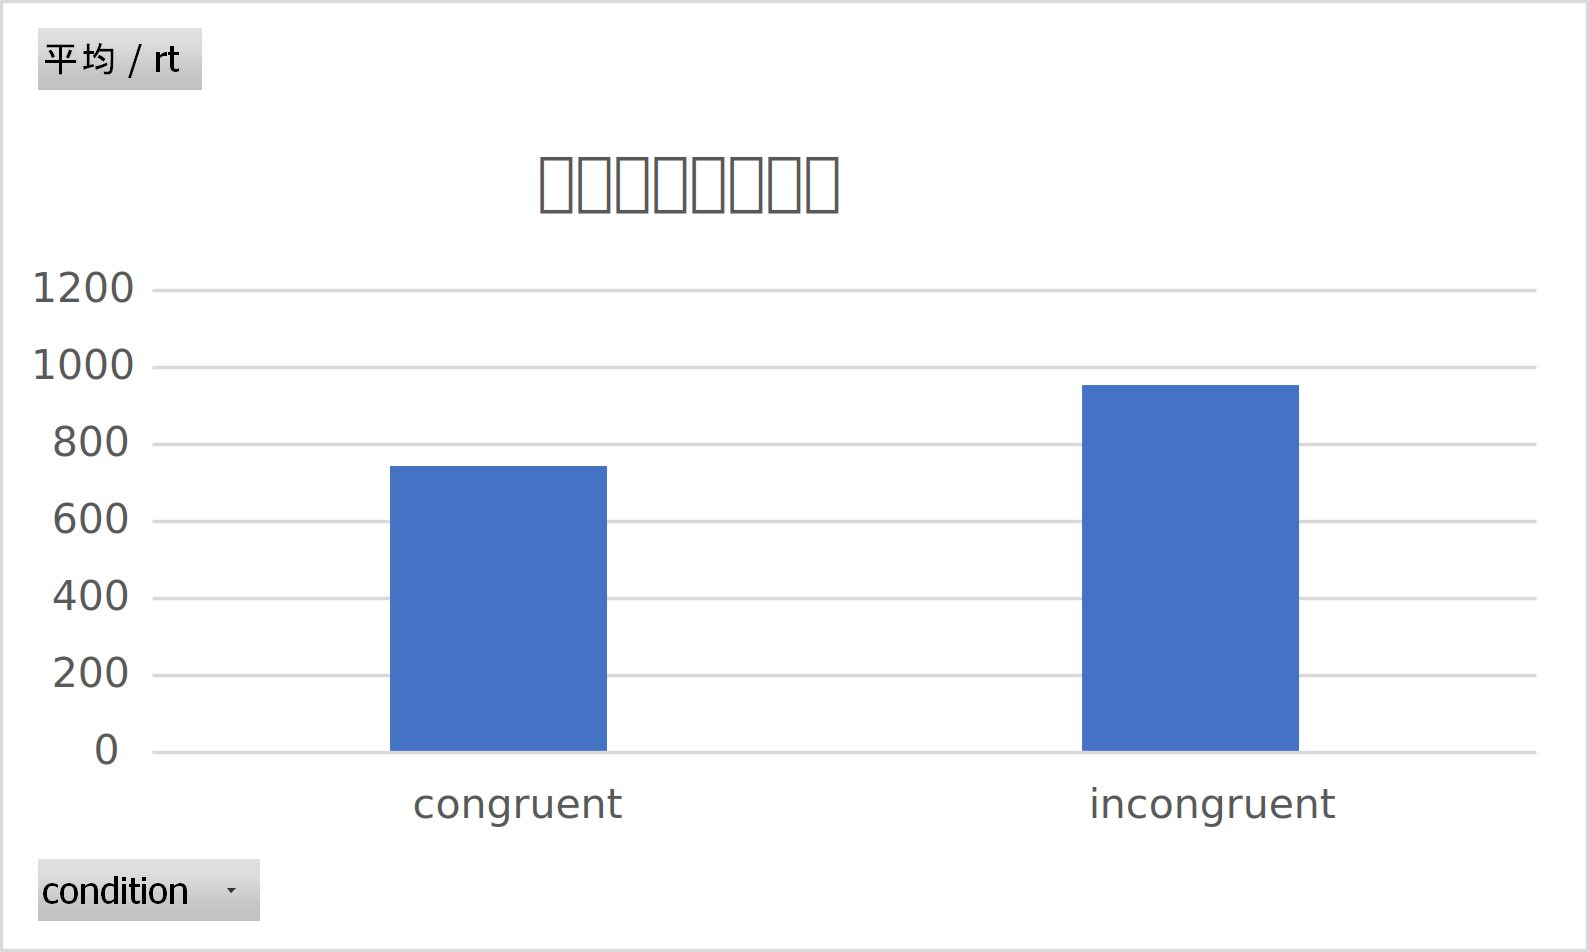
\includegraphics[width=0.6\linewidth]{ストループ効果.pdf}
    \caption{反応時間のグラフ}
    \label{fig:res_result}
  \end{figure}

  \begin{table}[htp]
    \centering
    \caption{ストループ課題の平均反応時間}
    \begin{tabular}{|l|r|} % l=左寄せ, r=右寄せ。| は縦線。
      \hline
      condition & 平均 / rt \\ \hline \hline
      congruent & 743.6315789 \\ \hline
      incongruent & 954.25 \\ \hline
    \end{tabular}
  \end{table}

  結果は以上の様になった.これはあくまで自分自身のみの結果であるが.結果は,単語の意味と色が一致しているときの方が不一致の場合に比べて,色を答えるのにかかる時間が短いことがわかった.

  \subsection*{第$2$回}
  行ったデータ分析の結果を以下に示す.この時,データ量は$18$人となっている.また,データ分析は\verb|Excel|で行っている.この検定は反応時間の平均に差があるかどうかを検定である.
  
  \begin{figure}[hbp]
    \centering
    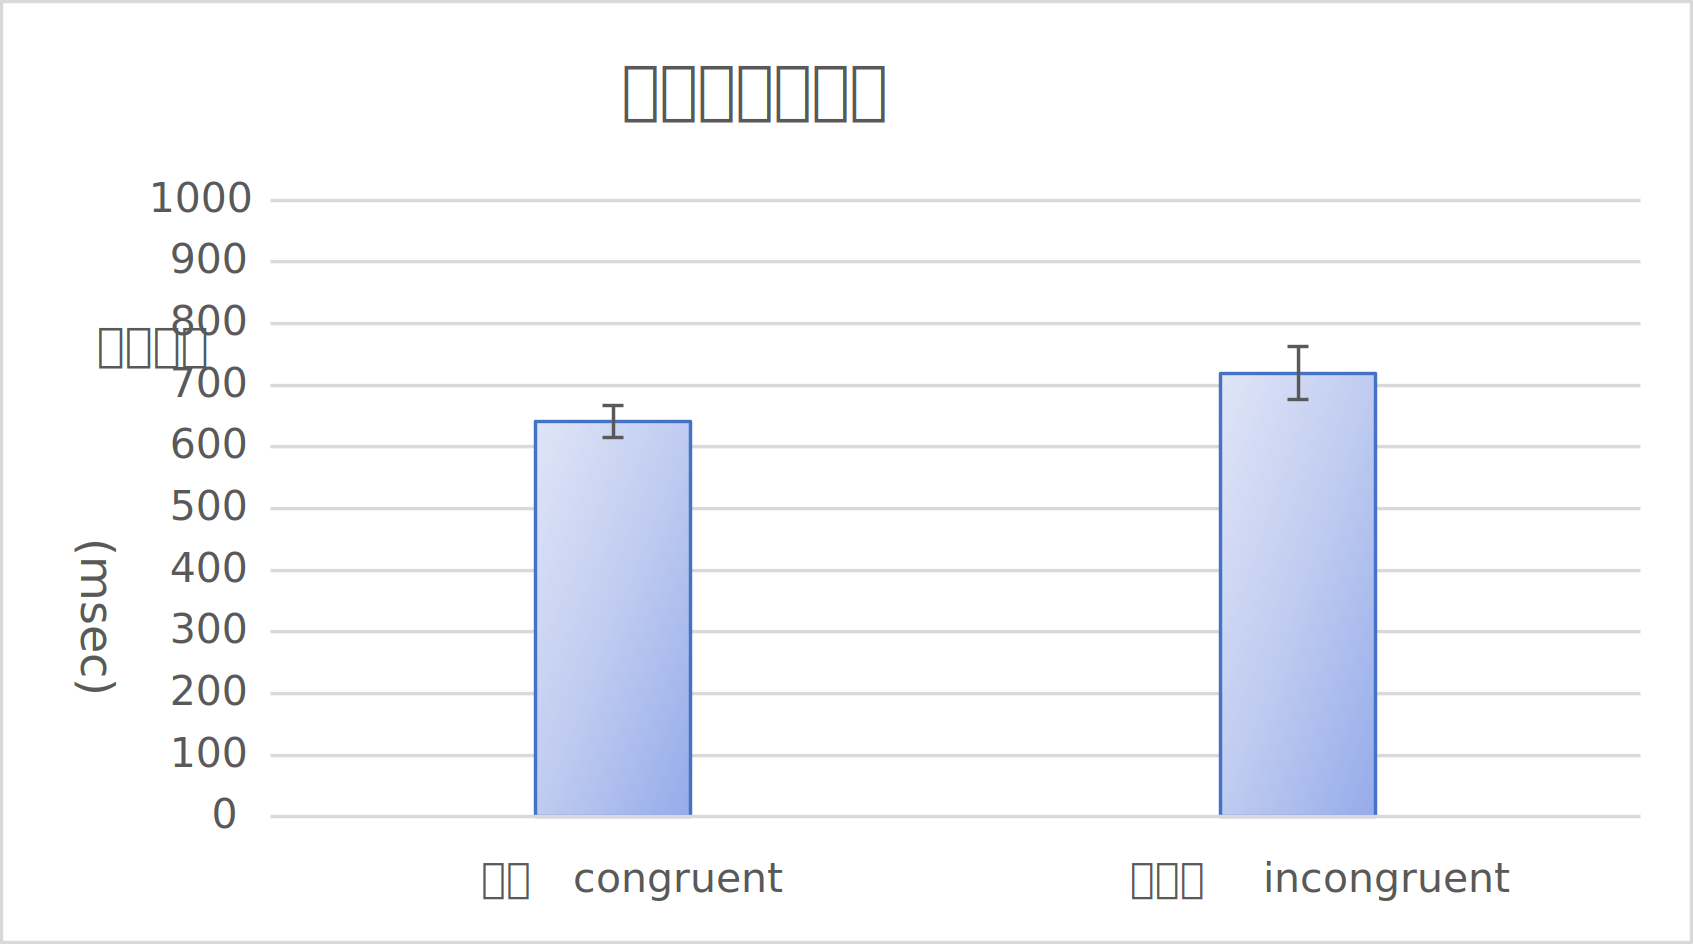
\includegraphics[width=0.6\linewidth]{t値.pdf}
    \caption{データ分析の結果}
    \label{fig:data_result}
  \end{figure}

  
  \begin{table}[htbp]
    \centering
    \caption{基本統計量(一致・不一致・差)}
    \begin{tabular}{|l|r|r|r|}
      \hline
      & \multicolumn{1}{c|}{一致} & \multicolumn{1}{c|}{不一致} & \multicolumn{1}{c|}{差} \\ \hline
      平均値 & 641.1666667 & 719.6666667 & 79.05555556 \\ \hline
      (不偏)分散 & 12008.26471 & 33827.17647 & 10925.82026 \\ \hline
      標準偏差 & 109.5822281 & 183.9216585 & 104.5266486 \\ \hline
      標準誤差 & 25.82877885 & 43.35075065 & 24.63716734 \\ \hline
    \end{tabular}
  \end{table}

  \begin{table}[htbp]
    \centering
    \label{data_graph}
    \caption{対応のある$t$検定の結果}
    \begin{tabular}{|l|r|}
      \hline
      $t$ 値 & 3.209 \\ \hline
      \multicolumn{2}{c}{} \\ \hline
      & 有意確率 ($p$) \\ \hline
      TDIST (両側) & 0.0051 \\ \hline
      T.TEST & 0.0054 \\ \hline
    \end{tabular}
  \end{table}

  \newpage

  \subsection*{第$3$回}
  \label{three}
  私たちは,\verb|Web|ページのユーザが行う主観評価の項目を``UIの可読性が高い''という評価に決定した.

  また,参考した\verb|Web|ページにはいくつか問題が存在したように感じる.それを以下に列挙する.
  \subsubsection*{サイトA}
  \begin{enumerate}[(1). ]
    \item 検索欄が少し,複雑であり初めて利用したユーザが使いづらい可能性がある.
    \item 最初のメインページでは,選択できる項目が少し少ない.
  \end{enumerate}

  \subsubsection*{サイトB}
  \begin{enumerate}[(1). ]
    \item 宿泊地を詳細にしか検索できず,大雑把に決めたい人にとって不便.
    \item $2$人,$2$部屋で予約すると,$1$人$1$部屋の料金しか表示されない.
  \end{enumerate}
  
  \subsubsection*{サイトC}
  \begin{enumerate}[(1). ]
    \item \verb|Web|ページの表示が遅い.
    \item 最初のページに表示される情報量が少ない.
  \end{enumerate}

  \subsubsection*{サイトD}
  \begin{enumerate}[(1). ]
    \item 最初のメインページに表示される情報量が多すぎる.
    \item 最初のメインページに表示される風景の情報が写真のみ.
  \end{enumerate}

  \subsection*{第$4$回}
  この主観評価について,\verb|Wilcoxon|の符号順位検索で検定する.

  以下の$3$つについて有意的な差みられたかどうか検定する.
  \begin{enumerate}[1. ]
    \item このサイトの見た目はスッキリしていて見やすい。
    \item このサイトは統一感がある.
    \item UIの可読性が高い.
  \end{enumerate}
  \begin{table}[htbp]
    \centering
    \caption{データ分析結果の有意確率 ($p$)}
    \label{data_3_result}
    \begin{tabular}{|l|c|l|c|}
      \hline
      課題1 & $p$ & & $p$ \\ \hline
      設問1(ab) & 0.000393 & 設問1(cd) & 0.052 \\ \hline
      設問2(ab) & 0.03799 & 設問2(cd) & 0.004017 \\ \hline
      設問3(ab) & 0.03988 & 設問3(cd) & 0.1595 \\ \hline
    \end{tabular}
  \end{table}

  この結果のグラフは付録に記載する.

  また,``このサイトを今後も利用したい''という$2$件法の項目についての$\chi ^ 2$検定の結果を以下に示す.

  \begin{table}[H]
    \centering
    \caption{サイトAとサイトBにおける回答の$\chi ^2 $検定}
    \label{chi_dataAB}
    \begin{tabular}{lrrr}
      \toprule
      サイト & はい & いいえ & 合計 \\
      \midrule
      サイトA & 60 (58.5) & 31 (32.5) & 91 \\
      サイトB & 57 (58.5) & 34 (32.5) & 91 \\
      \midrule
      合計 & 117 & 65 & 182 \\
      \bottomrule
      \multicolumn{4}{l}{\small ※( )内は期待値。$\chi^2(1) = 0.215, p = .643$}
    \end{tabular}
  \end{table}

  \begin{table}[H]
    \centering
    \caption{サイトC・Dにおける回答の$\chi ^ 2$ 検定}
    \label{chi_dataCD}
    \begin{tabular}{lrrr}
      \toprule
      サイト & はい & いいえ & 合計 \\
      \midrule
      サイトC & 63 (64.5) & 28 (26.5) & 91 \\
      サイトD & 66 (64.5) & 25 (26.5) & 91 \\
      \midrule
      合計 & 129 & 53 & 182 \\
      \bottomrule
      \multicolumn{4}{l}{\small ※( )内は期待値。$\chi^2 = 0.240, df = 1, p = .625$}
    \end{tabular}
  \end{table}

  

  \subsection{第$5$回}
  ユニバーサルデザインについては以下のようなグラフになるように修正した.
  \begin{figure}[hbp]
    \centering
    \includegraphics[width=0.6\linewidth]{cirlcle.png}
    \caption{折れ線グラフ}
    \label{fig:line}
  \end{figure}

  \begin{figure}[hbp]
    \centering
    \includegraphics[width=0.6\linewidth]{circle_after.png}
    \caption{円グラフ}
    \label{fig:circle}
  \end{figure}

  \section{考察}
  \subsection*{第$1$回}
  図\ref{fig:res_result}の結果から,``congruent'': 一致と``incongruent'': 不一致には約$100$平均/$rt$の差があることがわかった.このデータは自分自身のみのデータであるが,この結果から色と意味が一致する単語のほうが反応時間が早いことがわかる.

  \subsection*{第$2$回}
  表\ref{data_graph}より,データ数$n$より平均時間と誤差範囲にいくつかの差があることがわかる.また,図\ref{fig:data_result}からわかるように標準偏差にも差があることがわかる.これにより,データからみても差があることがわかる.

  また,表\ref{data_graph}より,$t$値が3.2から平均の差が標準誤差の$3.2$倍あるということになる.また,TDISTが$0.0051$,T.TESTが$0.0054$であることから,有意水準である$0.05$を大きく下回っている.よって,帰無仮説は棄却され,対立仮説が採択される.よってこのデータには有意な差があることがわかる.

  \subsection*{第$3$回}
  \ref{three}節より,これらの項目がユーザの体験を阻害していると判断した.

  \subsection*{第$4$回}
  表\ref{data_3_result}, \ref{chi_dataAB}, \ref{chi_dataCD}の結果から帰無仮説は以下のようになる.
  \begin{table}[htbp]
    \centering
    \caption{各検定における帰無仮説の判定結果 ($\alpha = 0.05$)}
    \label{data_kentei}
    \begin{tabular}{lrcl}
      \toprule
      検定対象 & 有意確率 ($p$) & 判定 & 備考 \\
      \midrule
      ストループ課題 ($t$検定) & 0.005 & 棄却される & 有意な差あり \\
      \midrule
      設問1(ab) & 0.000393 & 棄却される & 有意な差あり \\
      設問1(cd) & 0.052 & 棄却されない & 有意な差なし \\
      設問2(ab) & 0.03799 & 棄却される & 有意な差あり \\
      設問2(cd) & 0.004017 & 棄却される & 有意な差あり \\
      設問3(ab) & 0.03988 & 棄却される & 有意な差あり \\
      設問3(cd) & 0.1595 & 棄却されない & 有意な差なし \\
      \midrule
      サイトA・B比較 ($\chi^2$検定) & 0.643 & 棄却されない & 有意な差なし \\
      サイトC・D比較 ($\chi^2$検定) & 0.625 & 棄却されない & 有意な差なし \\
      \bottomrule
    \end{tabular}
  \end{table}

  表\ref{data_kentei}から,サイトAとサイトBにはすべての項目で有意な差が見られた.しかし,サイトCとサイトDではサイトの統一感にのみ有意な差が見られた.また,$\chi ^ 2$検定で両サイトを$2$件法で比較した際,有意な差はなかった.

  \subsection{第$5$回}
  今回私たちは,図\ref{fig:line}と図\ref{fig:circle}のようなデザインで作成したが,それぞれのグラフについて色覚者は付録のような見え方になる.それぞれの色についても見えやすく,それぞれの領域について白の線で分けることによってより見えやすくなるようになっている.また,図\ref{fig:line}についてはそれぞれの線の形を正方形や三角形にすることによって区別をしやすくしている.

\begin{thebibliography}{99}  
  \bibitem{step} 統計学へのステップ,長畑 秀和,共立出版株式会社,2000年
  \bibitem{stroop} ストループ効果: 認知心理学からのアプローチ,嶋田 博行,培風館,1994年
  \bibitem{nonparametric} ノンパラメトリック法,村上 秀俊,朝倉書店,2015
\end{thebibliography}



\newpage
\appendix
\section*{付録:実験データ詳細}

% A_and_B シリーズの貼り付け
\includepdf[pages=-]{A_and_B(1).pdf}
\includepdf[pages=-]{A_and_B(2).pdf}
\includepdf[pages=-]{A_and_B(3).pdf}

% C_and_D シリーズの貼り付け
\includepdf[pages=-]{C_and_D(1).pdf}
\includepdf[pages=-]{C_and_D(2).pdf}
\includepdf[pages=-]{C_and_D(3).pdf}

\newpage

\newpage
\appendix
\section{付録:色覚多様性に配慮したグラフの検証}

% --- 円グラフ専用のページを開始 ---
\clearpage
\subsection{円グラフの比較(各色覚型での見え方)}
\begin{figure}[H]
  \centering
  % 上段:オリジナルと修正後の比較(大きめに配置)
  \hspace{0.05\linewidth}
  \begin{minipage}{0.45\linewidth}
    \centering \includegraphics[width=\linewidth]{circle_after.png}
    \caption{修正後(円)}
  \end{minipage}

  \vspace{5em} % 上段と下段の間の余白(1ページに収まるよう調整)

  % 下段:3つの色覚シミュレーション(横に3つ並べる)
  \begin{minipage}{0.31\linewidth}
    \centering \includegraphics[width=\linewidth]{circle_P.png}
    \caption{1型二色覚者}
  \end{minipage}
  \hfill
  \begin{minipage}{0.31\linewidth}
    \centering \includegraphics[width=\linewidth]{circle_D.png}
    \caption{2型二色覚者}
  \end{minipage}
  \hfill
  \begin{minipage}{0.31\linewidth}
    \centering \includegraphics[width=\linewidth]{circle_T.png}
    \caption{3型2色覚者}
  \end{minipage}
\end{figure}
\clearpage % ここで改ページして、円グラフだけのページを確定させる
% --- 円グラフのページ終了 ---

% --- 次のページから折れ線グラフを開始 ---
\subsection{折れ線グラフの比較(各色覚型での見え方)}
\begin{figure}[H]
  \centering
  % 上段:オリジナル(中央に配置)
  \includegraphics[width=0.6\linewidth]{line.png}
  \caption{オリジナル(線)}
  \label{fig:line_orig}

  \vspace{2em} % 上段と下段の間の隙間

  % 下段:3つのシミュレーションを横一列に配置
  \begin{minipage}{0.32\linewidth}
    \centering
    \includegraphics[width=\linewidth]{line_P.png}
    \caption{1型二色覚(図10)}
  \end{minipage}
  \hfill
  \begin{minipage}{0.32\linewidth}
    \centering
    \includegraphics[width=\linewidth]{line_D.png}
    \caption{2型二色覚(図11)}
  \end{minipage}
  \hfill
  \begin{minipage}{0.32\linewidth}
    \centering
    \includegraphics[width=\linewidth]{line_T.png}
    \caption{3型二色覚(図12)}
  \end{minipage}
\end{figure}

\end{document}
